\documentclass{article}
\usepackage{../../Self_Style}

\title{Phys 20AL Week 3: Pendulum Improvement}
\author{Zih-Yu Hsieh}
\date{\today}

\begin{document}
\maketitle

\section{Aim for Experiment}
The experiment is to measure the amplitude dependence of the pendulum's period, experimenting with how the maximum initial angle affects the period of the pendulum. It also aims for testing the accuracy of the provided formula, where with maximum angle $\theta_0$, the period formula is given as follow:
$$T(\theta_0)=2\pi\sqrt{\frac{l}{g}}\left(1+\frac{1}{16}\theta_0^2+\frac{11}{3072}\theta_0^4+...\right)$$ 

\section{Experimental Setup}
\subsection{Experiment with Electronic Detector}
Equipments include: Stand, Clamp, string, spherical mass, protractor, meter stick , detector, computer.

The following is the steps for setup:
\begin{itemize}
    \item[1.] Setup the stand at hte edge of the table.
    \item[2.] Tie one end of the string onto the clamp, pass the other end through the hole at the top of the stand, and clip the clamp onto the stand (to fix the length of the string as pendulum's arm).
    \item[3.] Fix the center of the protractor at the top of the stand at where the pivot of the pendulum is at.
    \item[4.] Fix the spherical mass at the free end of the string (treated as mass of the simple pendulum).
    \item[5.] Fix the detector at the bottom of the stand (the location slightly lower than the spherical mass's position) for ease to detect the period of the spherical mass.
\end{itemize}
\begin{figure}[h!]
    \centering
    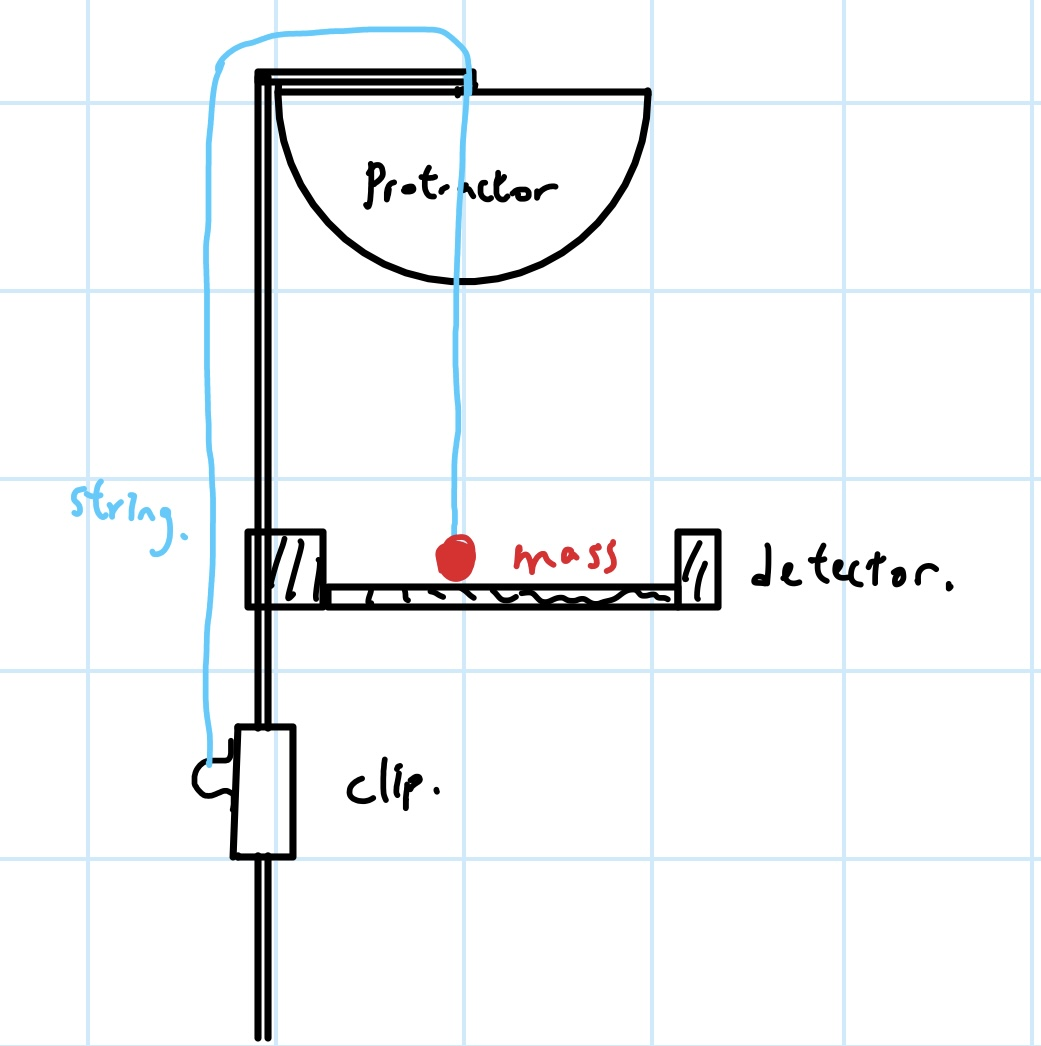
\includegraphics[width=80mm]{sketch_detector.jpg}
\end{figure}

\pagebreak

\subsection{Experimnt without Electronic Detector}
Equipments include: Stand, Clamp, string, spherical mass, protractor, meter stick , timer, phone (use as camera).

The setup is nearly identical with the previous one, except for not fixing a detector on the stand.
\begin{figure}[h!]
    \centering
    \includegraphics[width=80mm]{sketch_nodetect.jpg}
\end{figure}

\section{Measurement \& Method of Measure}
For each fixed manipulated variable we'll measure total of $5$ trials.

For both experiment, the manipulated variables are the maximum angle of the pendulum (recorded in degrees $ ^\circ$, and measured using protractor). In both experiments we experimented with angle $\theta=10^\circ, 20^\circ, 30^\circ, 40^\circ$, and $50^\circ$. 

The responding variable on the other hand is the time period of the pendulum under the given angle. In the two setups, the measurements are done differently:
\begin{itemize}
    \item For the setup with detector, the detector records the time when the pendulum passes through the lowest point, which serves as a recording of time period.
    \item For the setup without detector, it's setting up the timer in the background environment of the pendulum (let it run before starting the pendulum), and use the phone camera to record the whole pendulum process. Afterward, we'll check individual frames fo get a more precise measurement of the time period (which would be a lot more tedious, so it's not possible to include the data in this lab note).
\end{itemize}

\section{Collected Data (Setup with Detector only)}
\textbf{Rmk:} The other setup records time with video, which is a lot more time consuming to check and record the actual time period, which we'll not include here (since there's no time to finish it before the lab note is due).

\begin{figure}[h!]
    \centering
    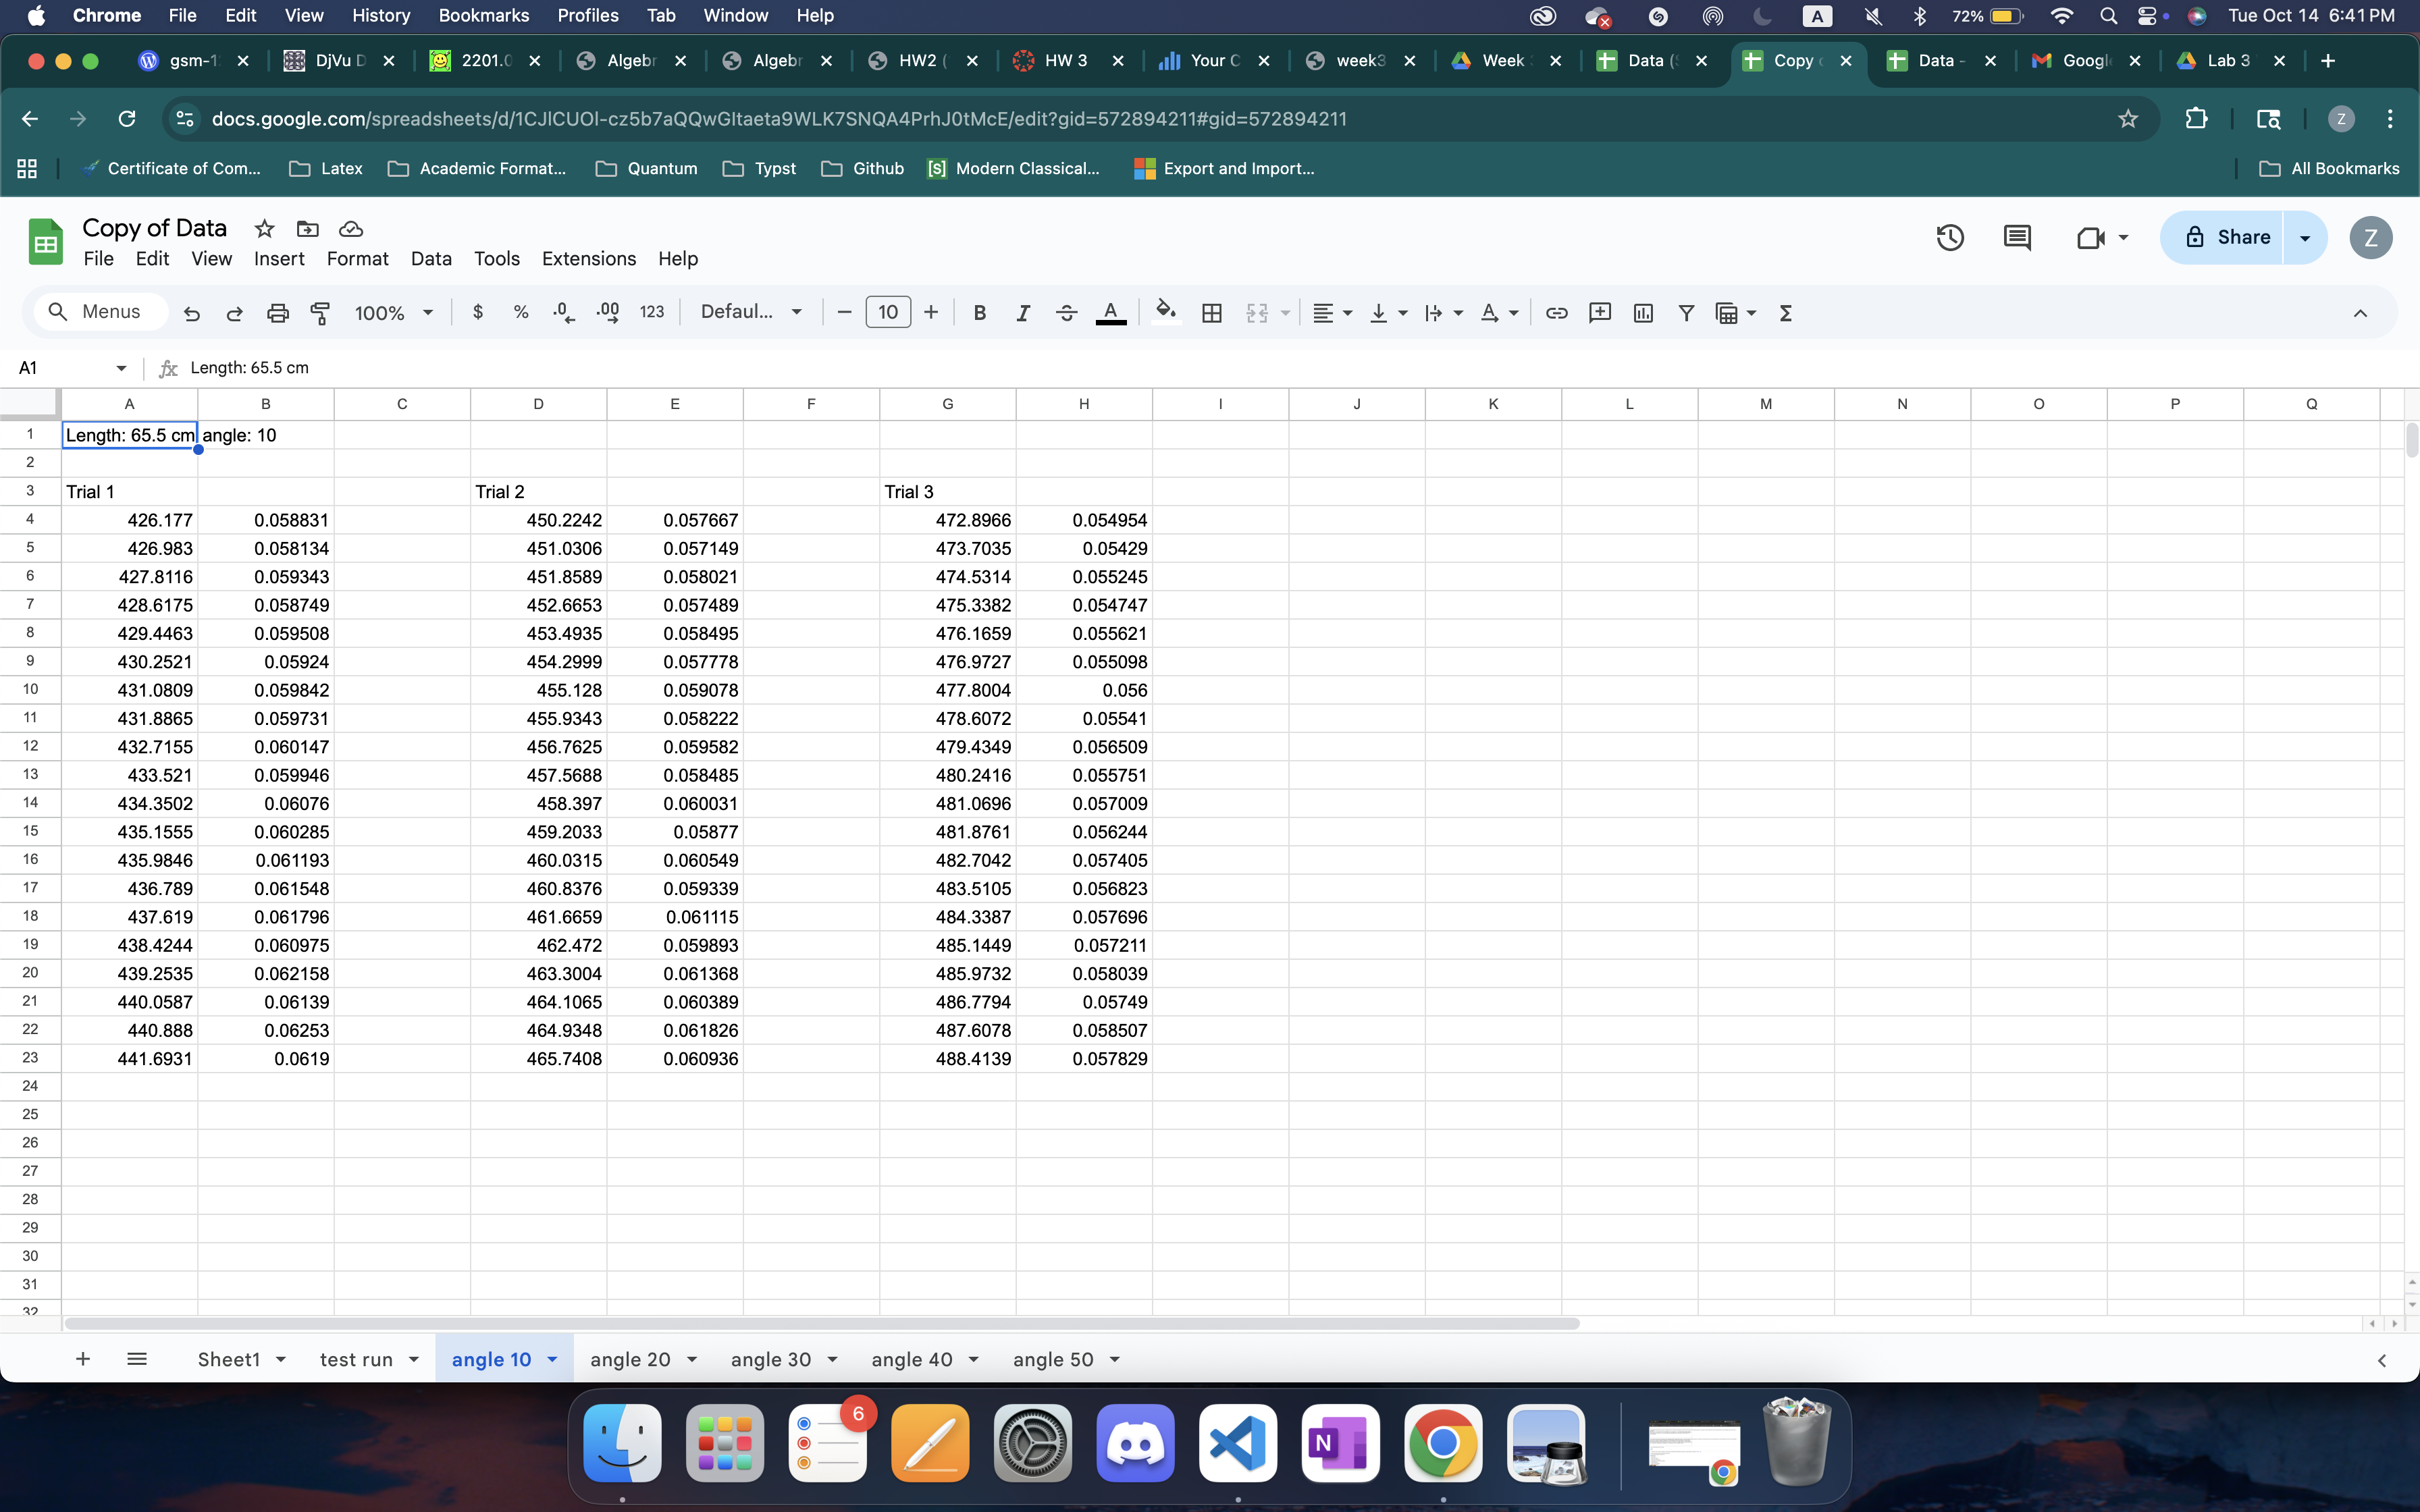
\includegraphics[width=150mm]{angle_10.png}
    \caption{Data for angle $10^\circ$}
\end{figure}
\begin{figure}[h!]
    \centering
    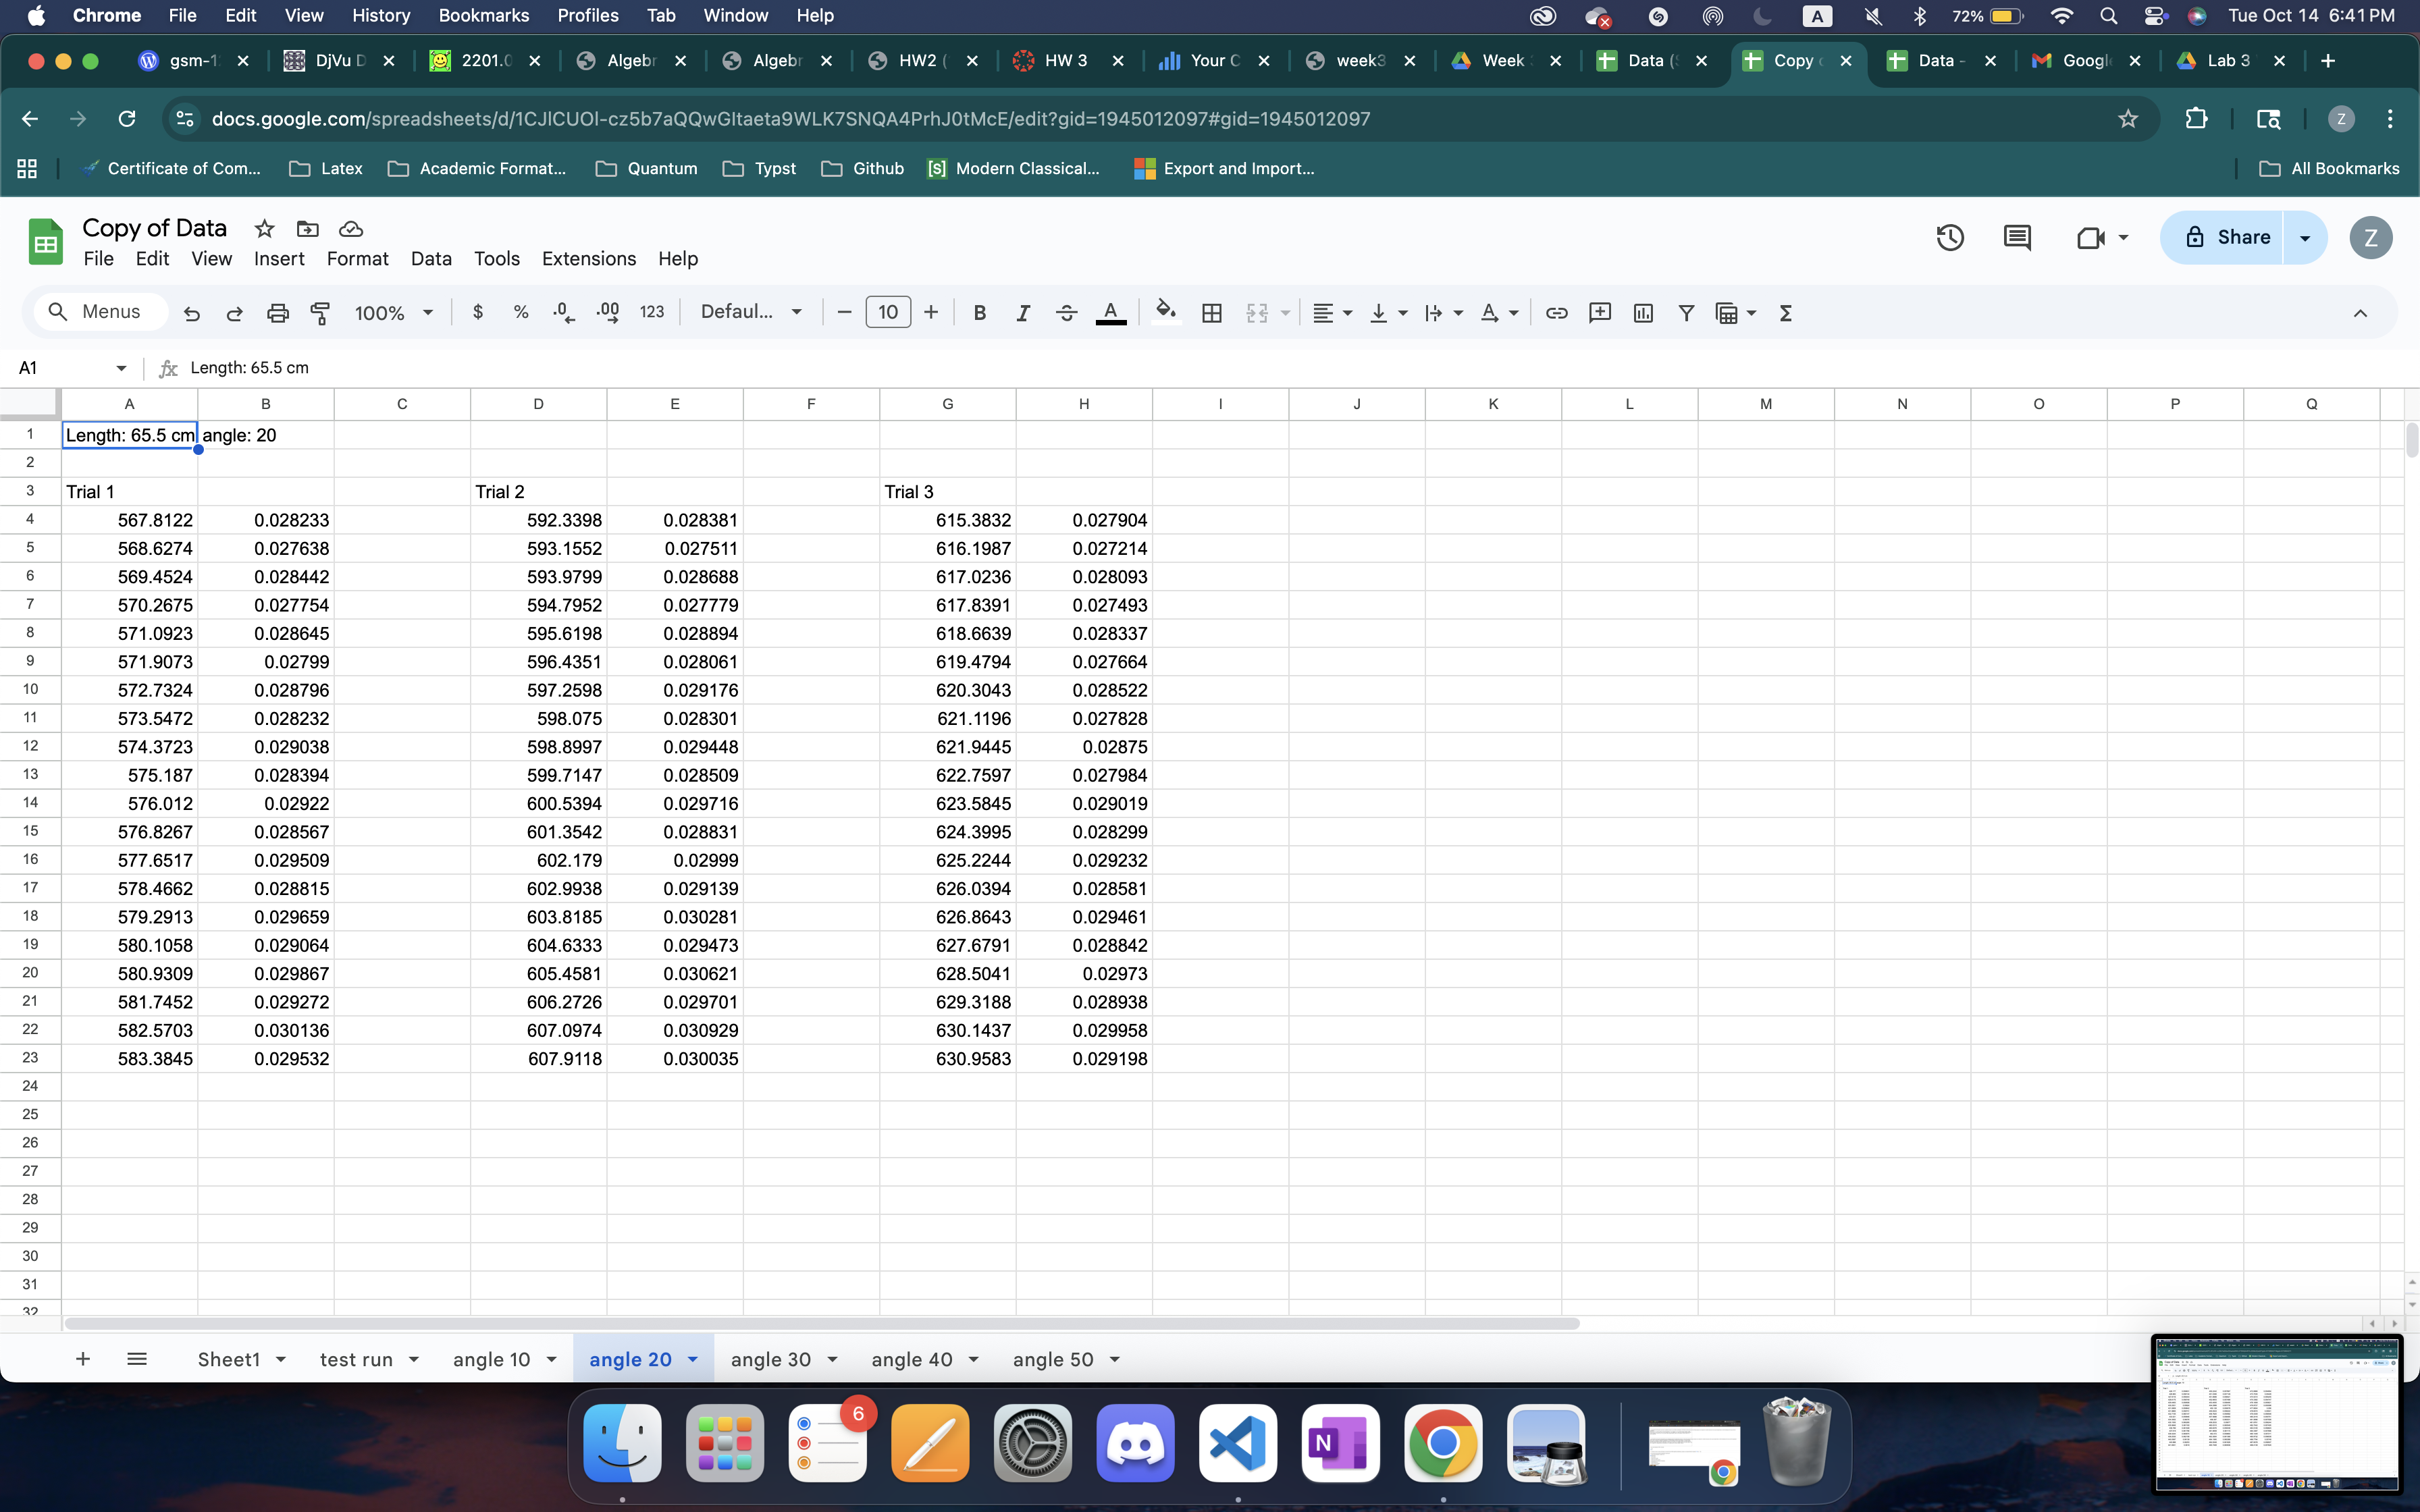
\includegraphics[width=150mm]{angle_20.png}
    \caption{Data for angle $20^\circ$}
\end{figure}
\begin{figure}[h!]
    \centering
    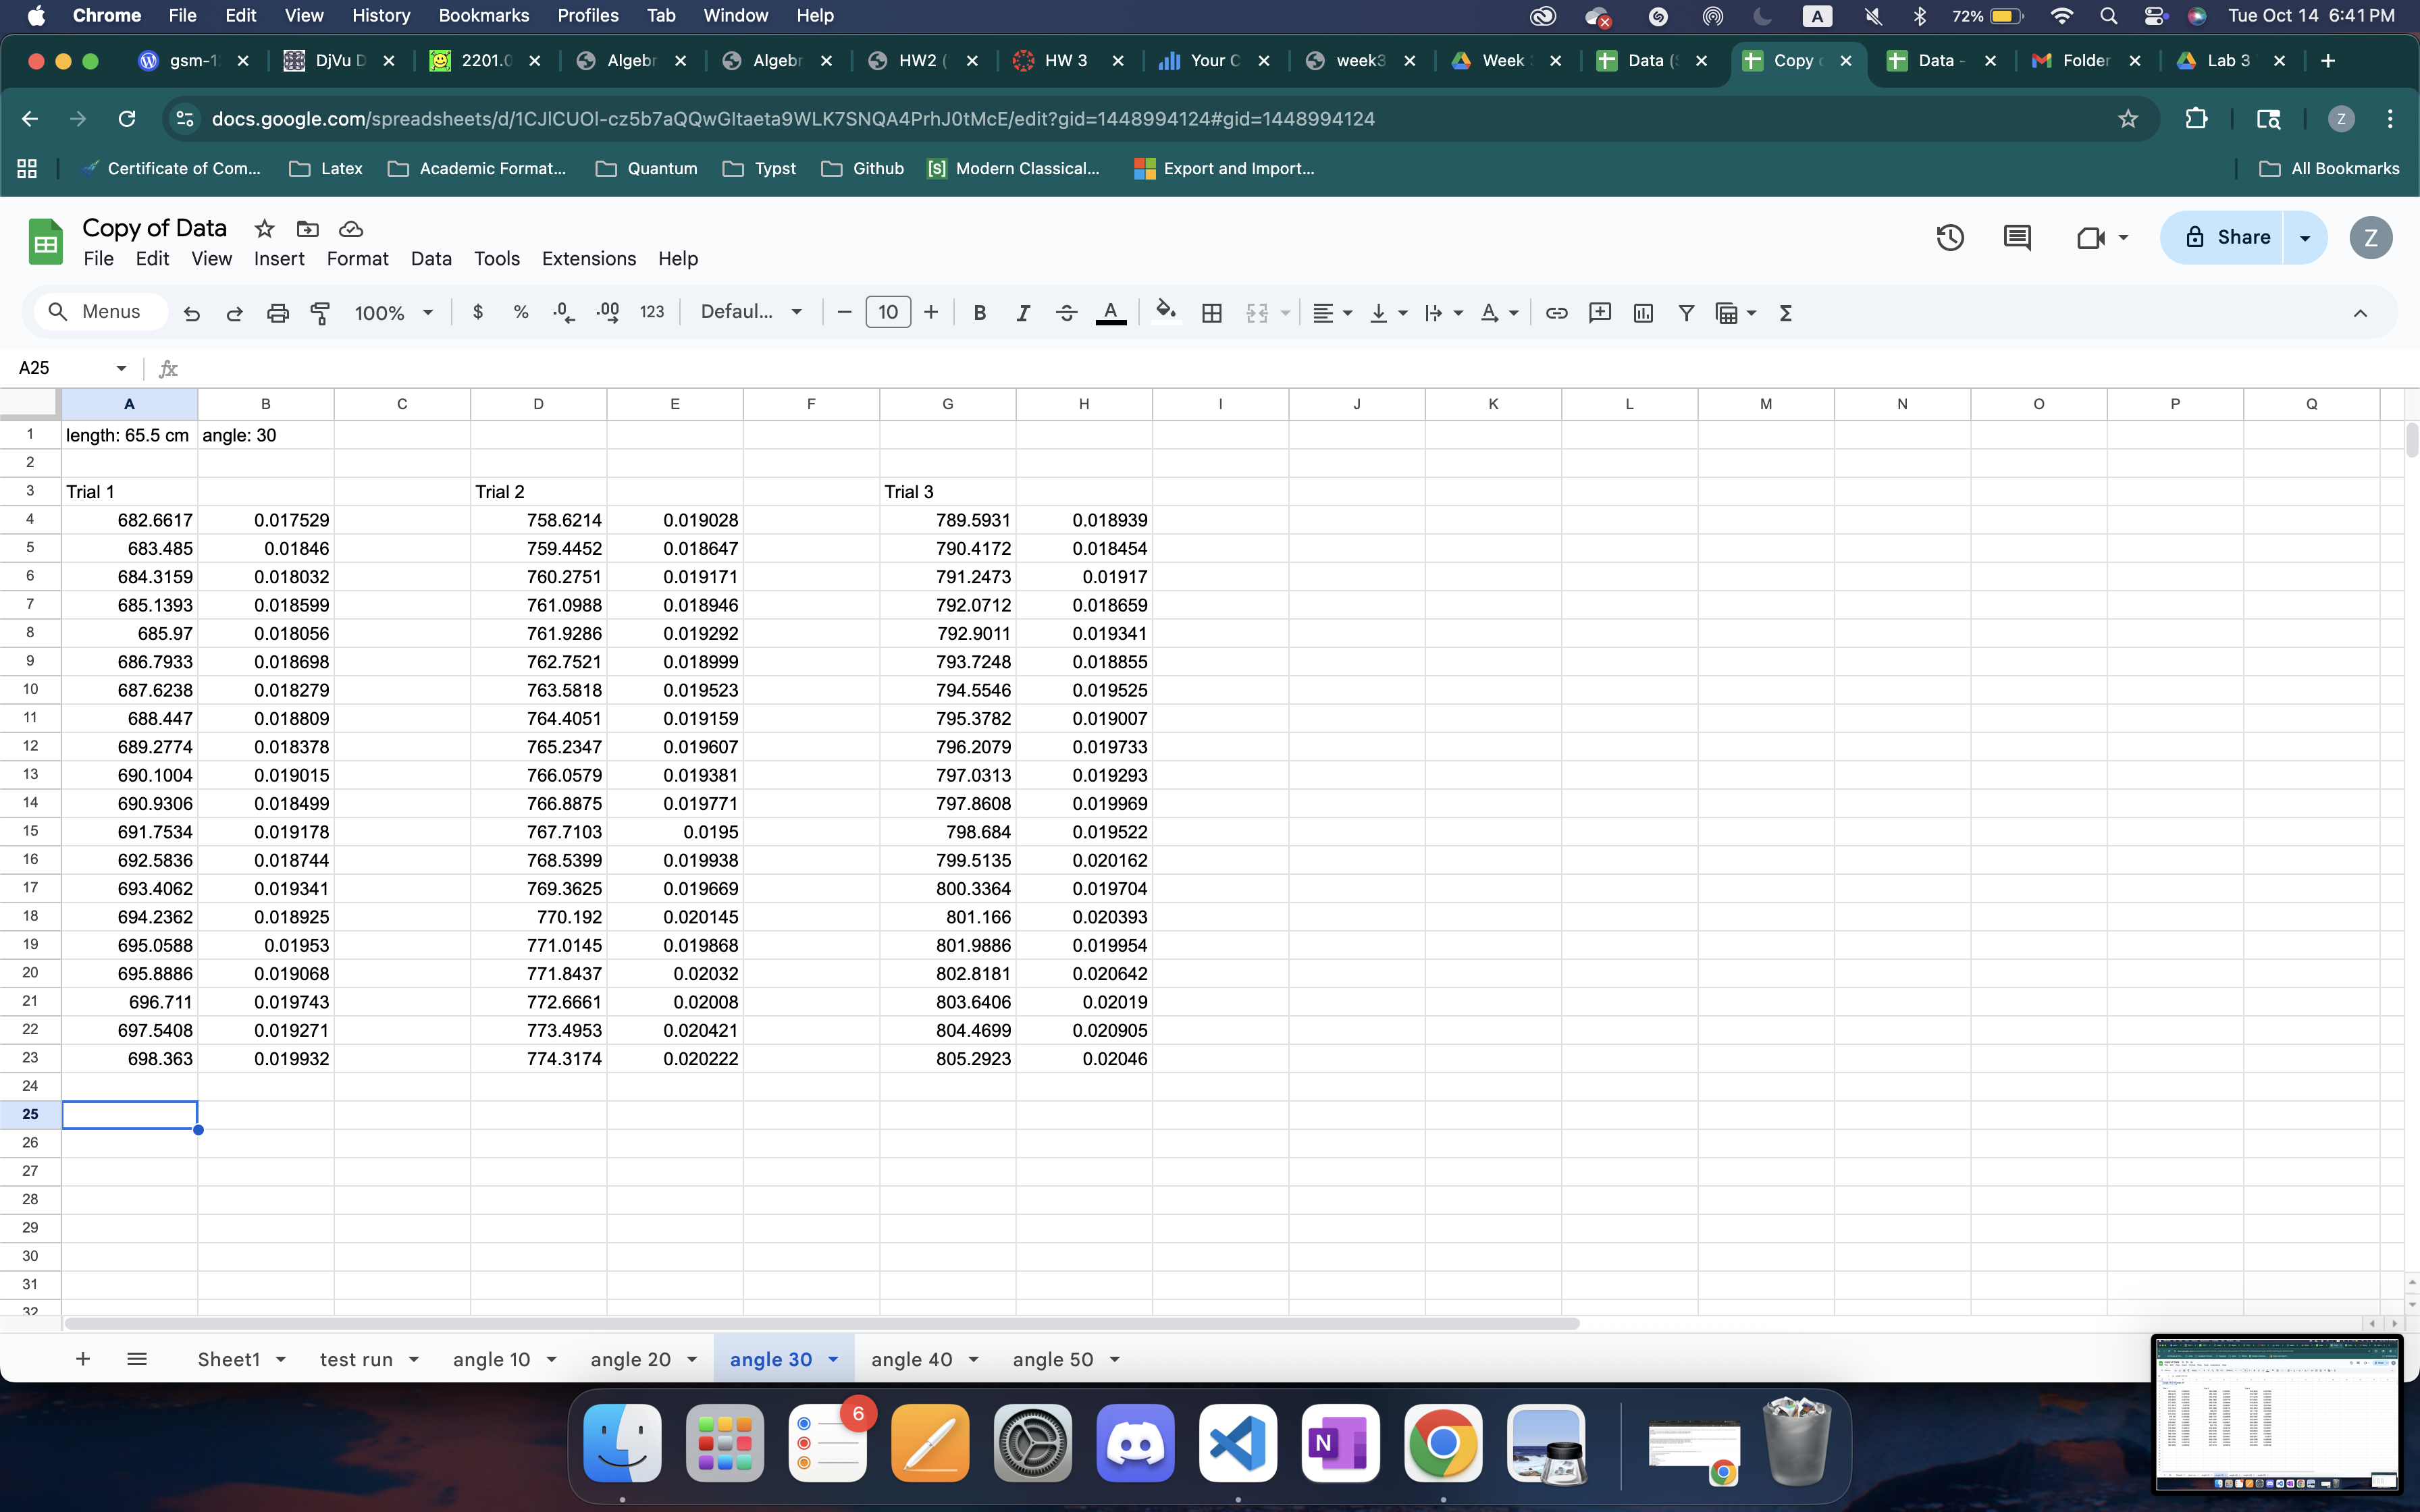
\includegraphics[width=150mm]{angle_30.png}
    \caption{Data for angle $30^\circ$}
\end{figure}
\begin{figure}[h!]
    \centering
    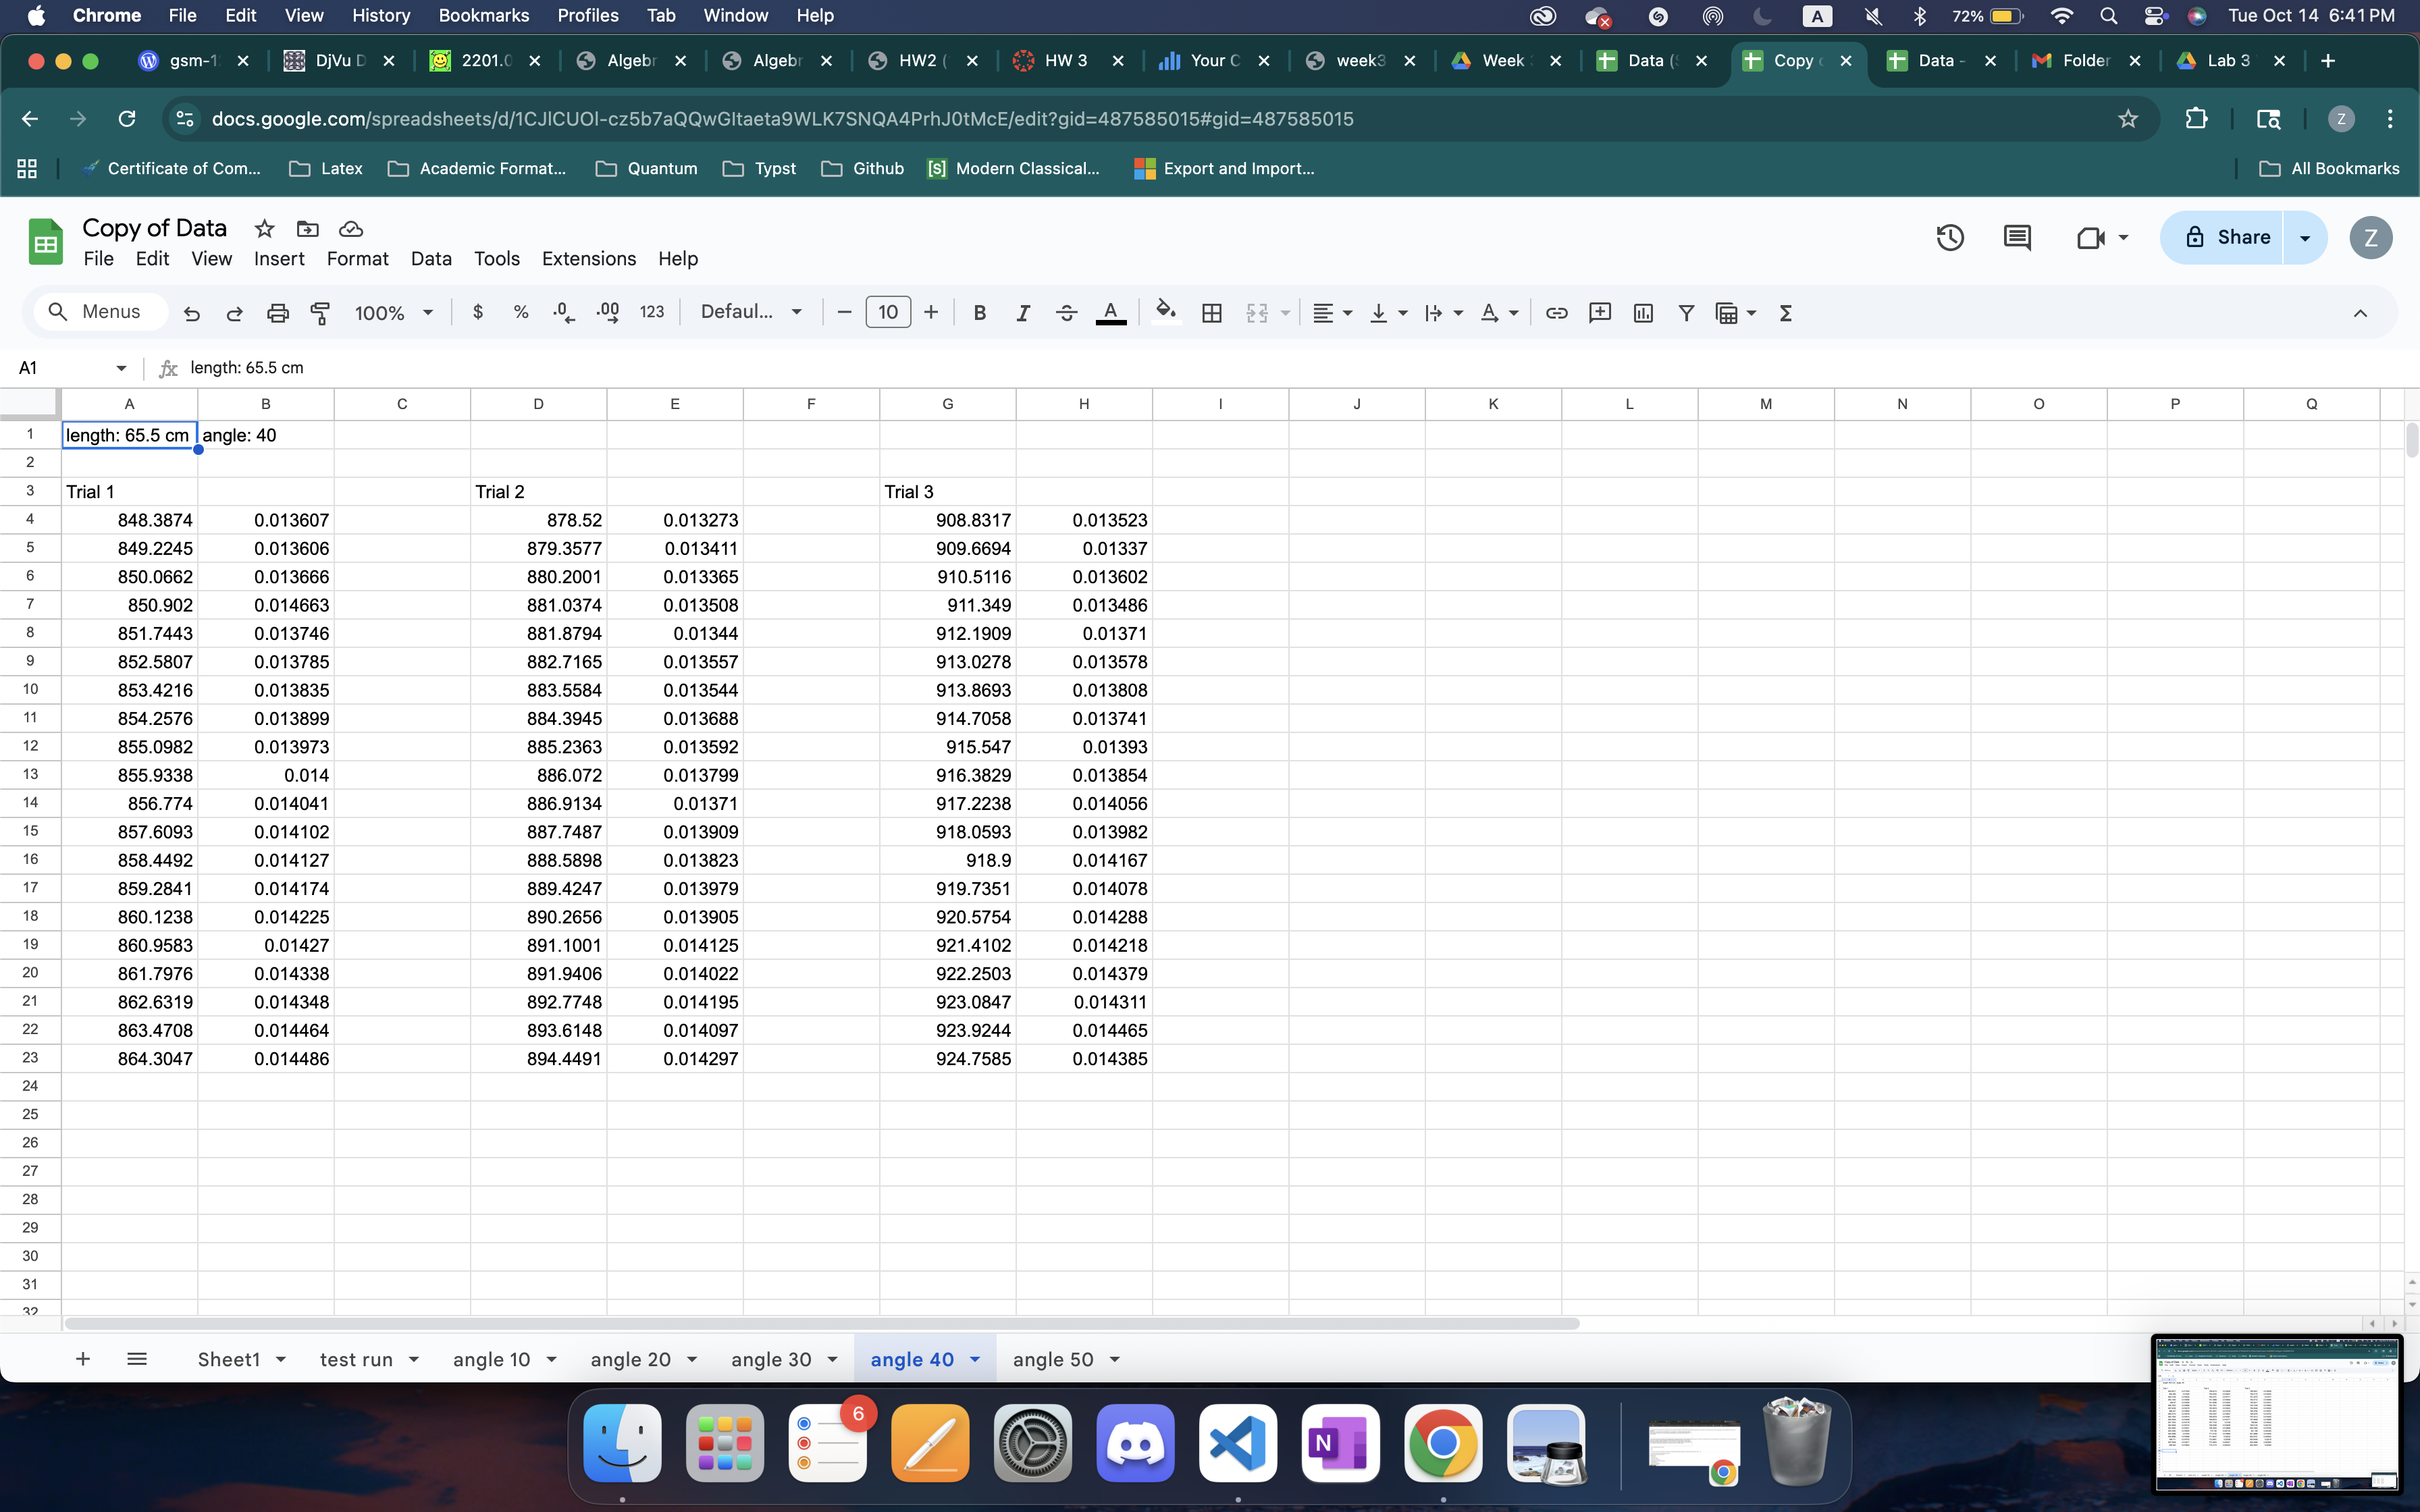
\includegraphics[width=150mm]{angle_40.png}
    \caption{Data for angle $40^\circ$}
\end{figure}
\begin{figure}[h!]
    \centering
    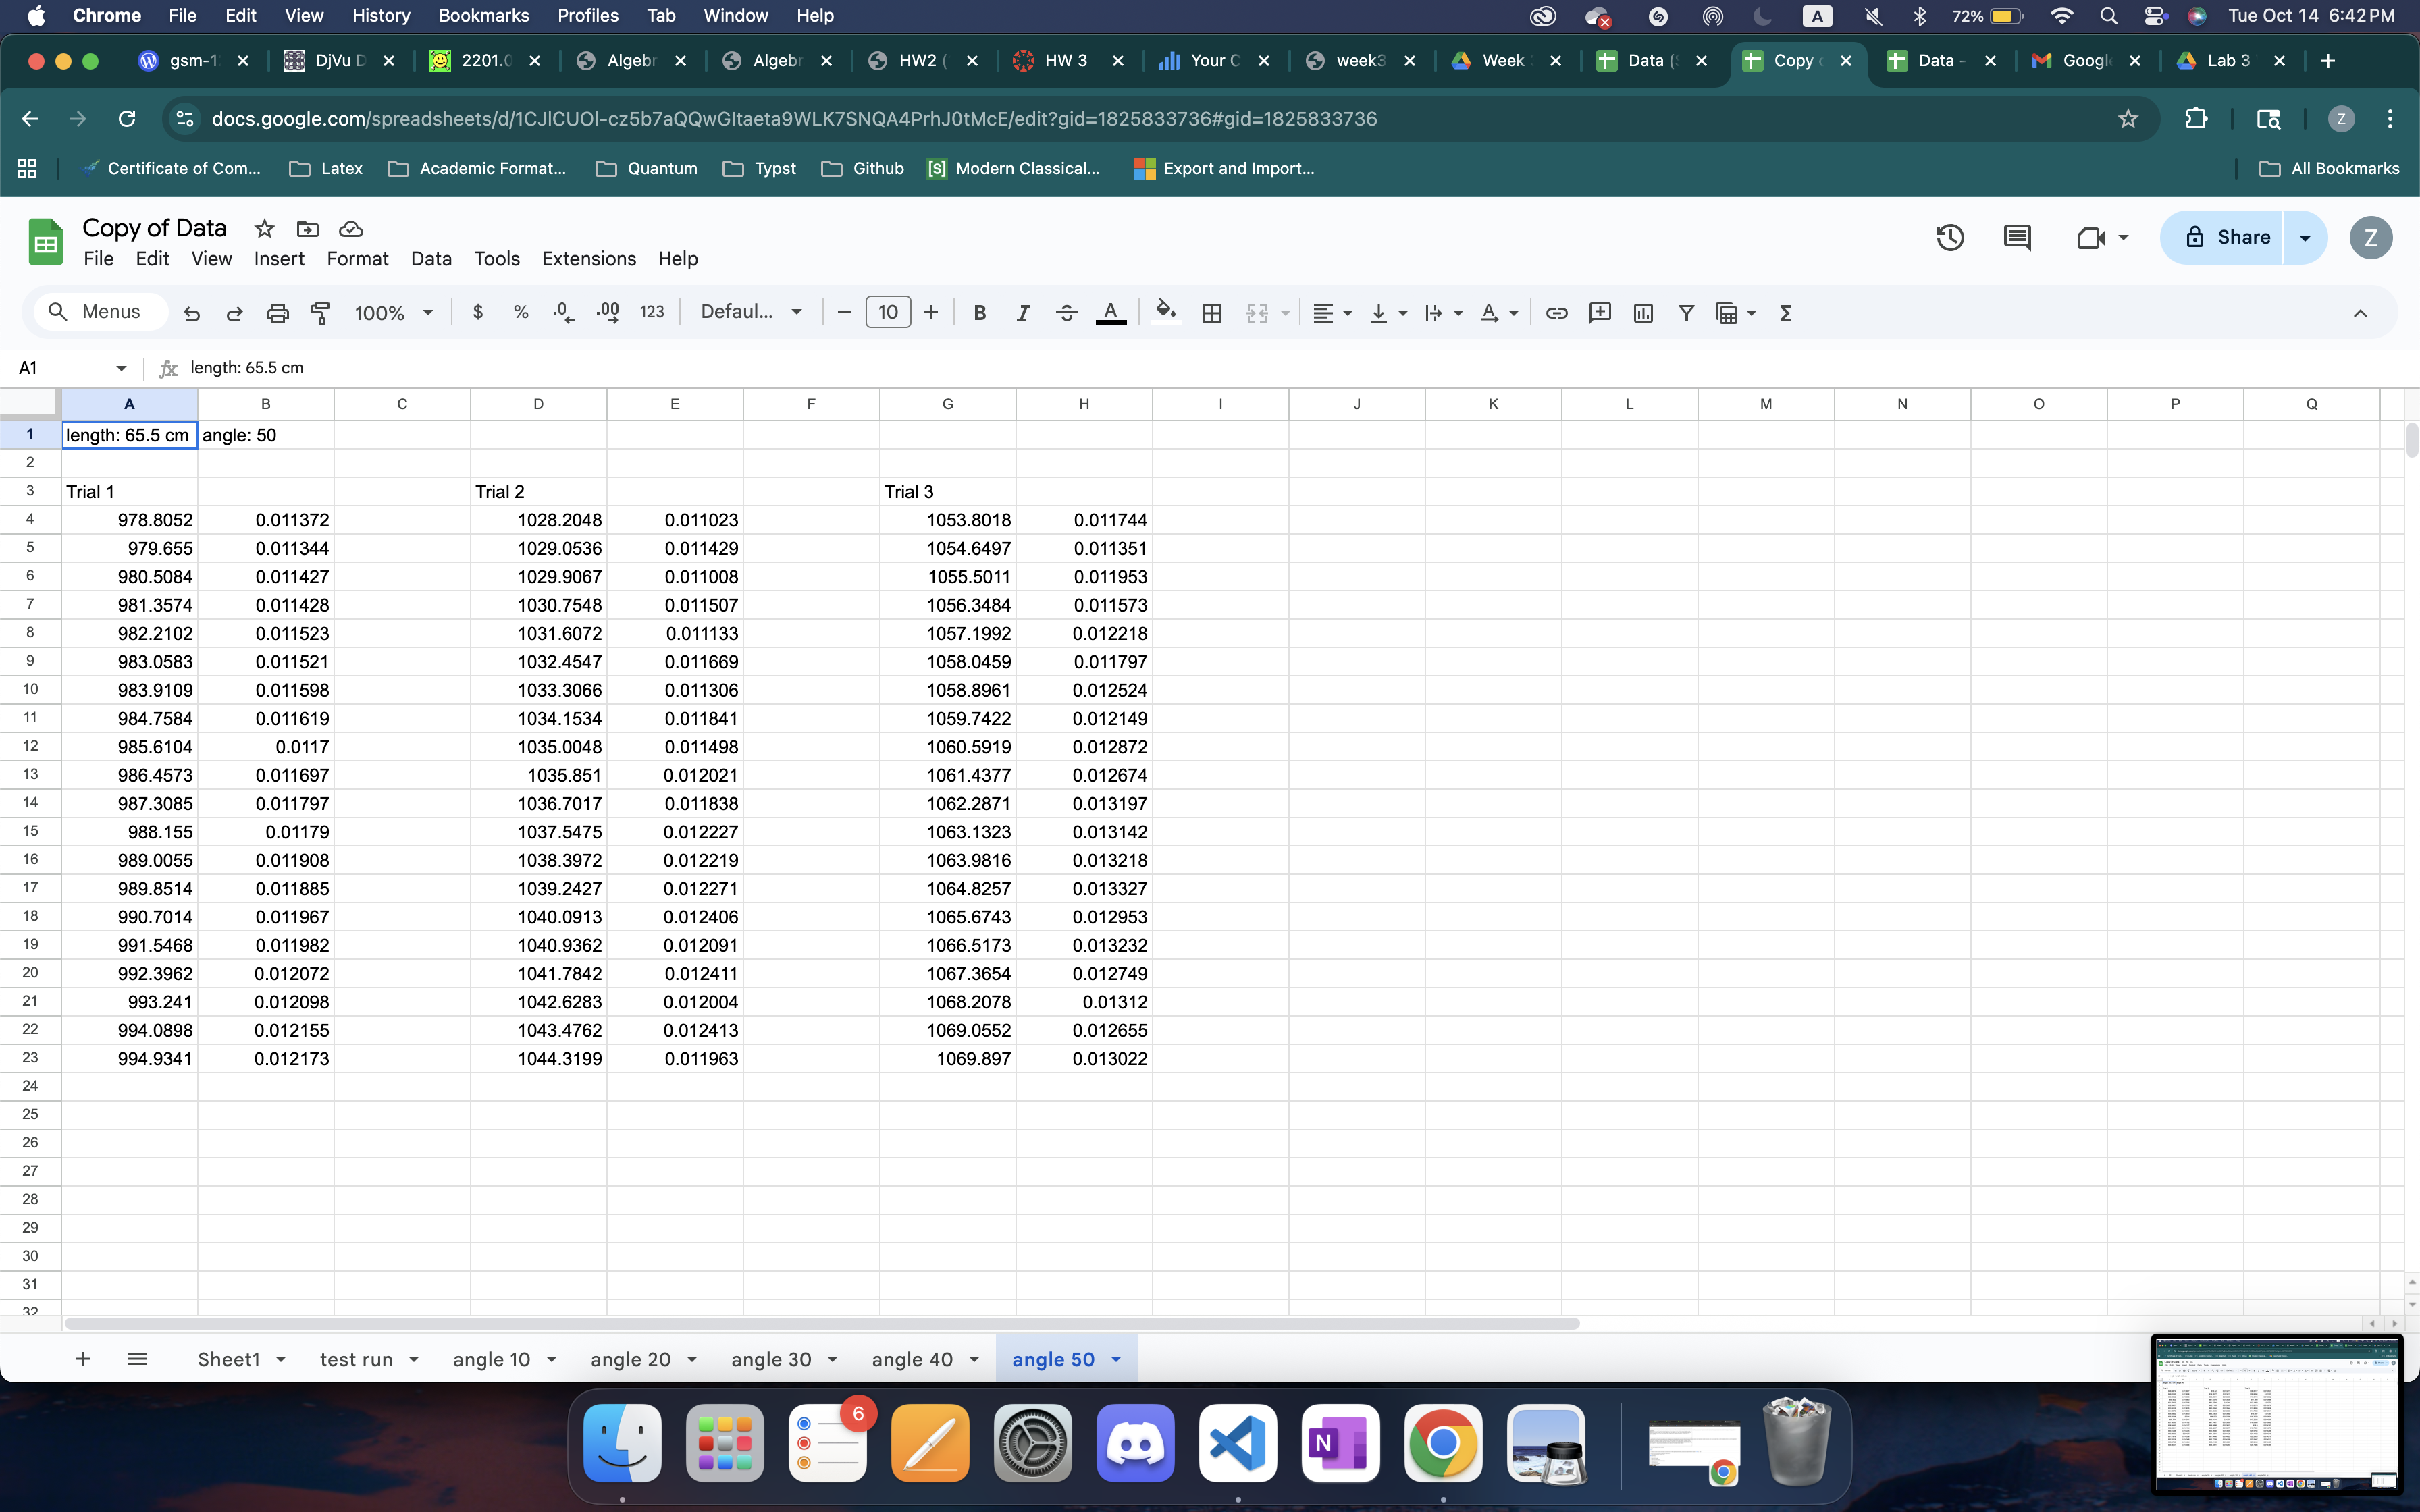
\includegraphics[width=150mm]{angle_50.png}
    \caption{Data for angle $50^\circ$}
\end{figure}
\begin{figure}[h!]
    \centering
    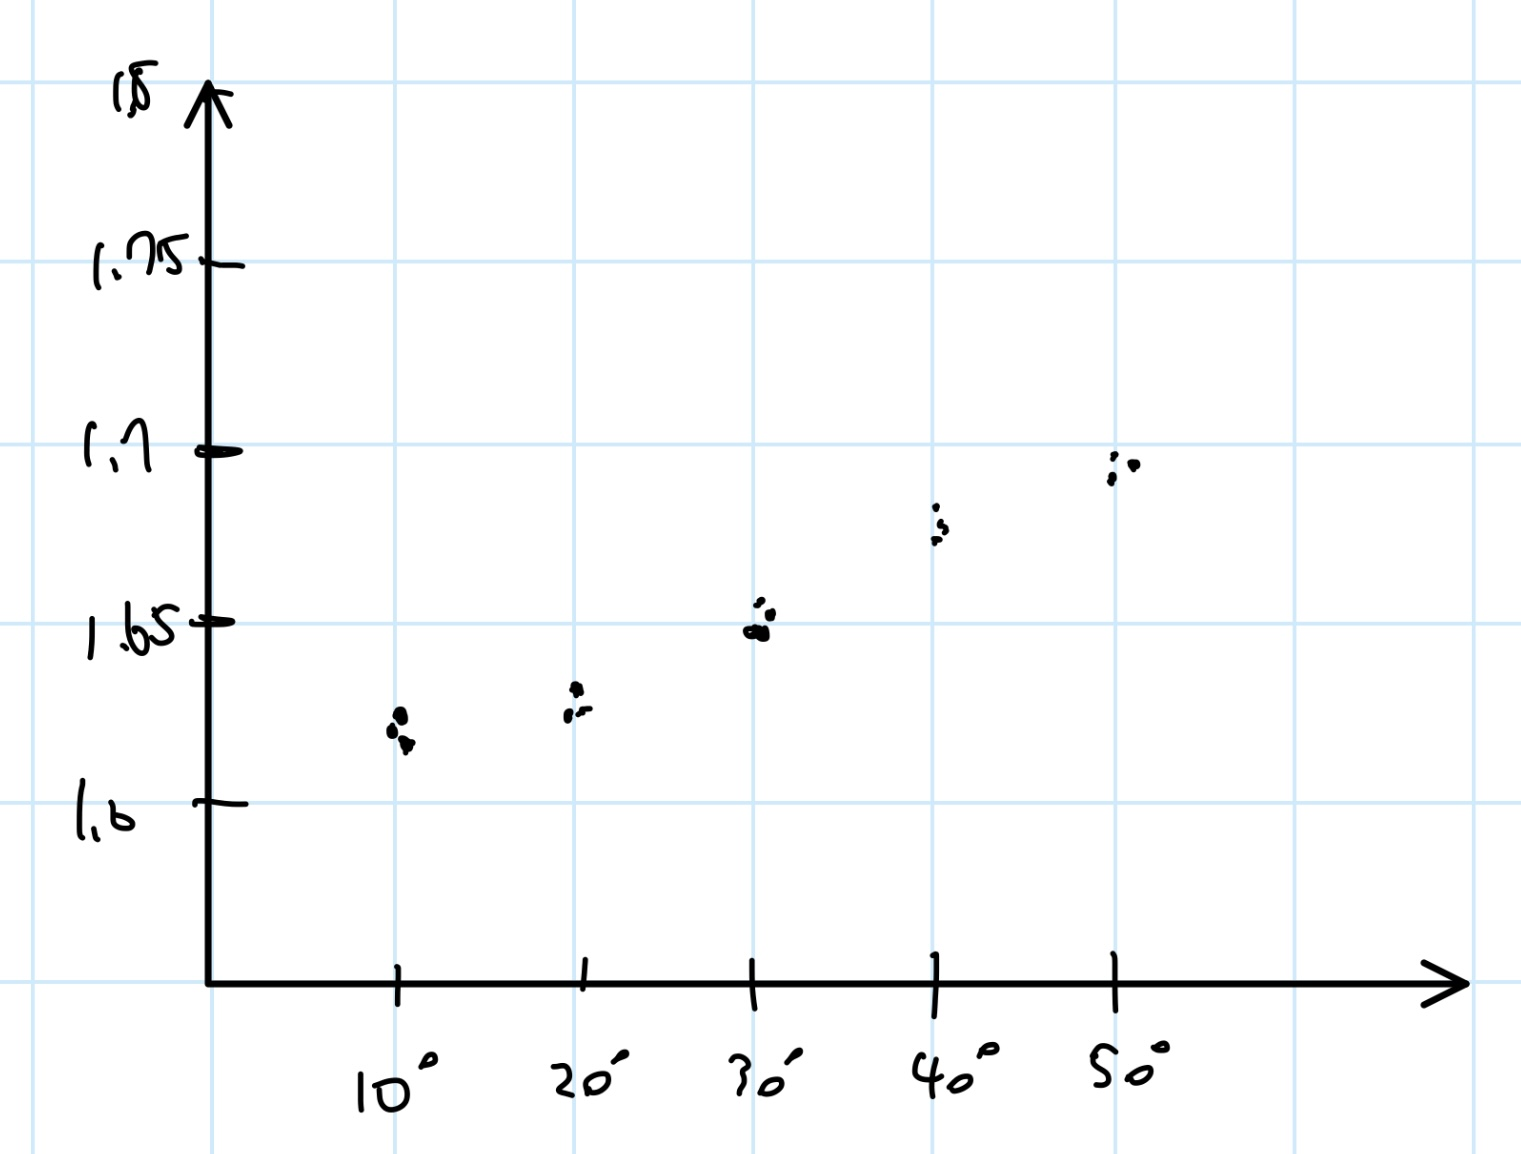
\includegraphics[width=150mm]{sketch_data.jpg}
    \caption{Sketch of the Data Table collecting the Average Time Period, with respect to Max Angle of the Pendulum}
\end{figure}


\end{document}